\documentclass[english]{article}

\usepackage{babel}
\usepackage{graphicx}
\usepackage{times}
\usepackage{pifont}
\usepackage[margin=1in]{geometry}
\usepackage{eurosym}
\usepackage{fancyhdr}
\usepackage[hidelinks]{hyperref}
\usepackage{float}

\pagestyle{fancy}
\fancyhf{}


%HEADER
%**************************************************************************************
\pagestyle{fancy}
\fancyhf{}
%**************************************************************************************
\lhead{Internship Report}		 	 
\rhead{Savonia University of Applied Sciences} 
\lfoot{EFA12SF}
\cfoot{\thepage}
\rfoot{Alexey Tukalo}
%**************************************************************************************

\date{}
\setlength\parindent{0pt}

\begin{document}

\title{\vspace{2in}INTERNSHIP REPORT\\
\small Savonia University of Applied Sciences\\
\vspace{0.5in}
\includegraphics{savonia.jpg}}

\nopagebreak
\maketitle


\vspace{3in}

\author{
\begin{flushleft}
Student name: Alexey Tukalo,\\
Student number: 67687,\\
Group: EFA12SF,\\
Type: The internship information technologies,\\
Duration: 4 months and 1 week or 720 hour (07.07.2015-18.11.2015)\\
The day of the report: \date{\today}
\end{flushleft}
}

\thispagestyle{empty}

\newpage
\setcounter{page}{1}
\setcounter{tocdepth}{2}
\tableofcontents

\newpage

%MAIN CONTENT ******************************************************************************************************************

\section{Company}

I have got my summer practice at Institute of Data Processing and Electronics, which belonges to the Karlsruhe Institute of Technology (KIT). The organisation's visitor address is Hermann-von-Helmholtz-Platz 1, 76344 Eggenstein-Leopoldshafen, Germany and mailing address is Karlsruhe Institute of Technology (KIT) - Campus North, Institute for Data Processing and Electronics (IPE), P.O. Box 3640, 76021, Karlsruhe, Germany. The phone number is +49 721 608 2 2027, an e-mail address is info@ipe.kit.edu, ipe.kit.edu is the webpage of the organisation. I worked under supervision of Dr. Torsten Hopp, his e-mail address is torsten.hopp@kit.edu and the phone number is +49 721 608-25990. The internship period is from the 7th of July to the 18th of November.

\subsection{General Information}

Karlsruhe Institute of Technology is one of the larges research and education organisation in Germany. In 2009, University of Karlsruhe\footnote{Founded in 1825} merged with Karlsruhe Research Center Forschungszentrum Karlsruhe\footnote{Based on national nuclear research center opened in 1956 and called Kernforschungszentrum Karlsruhe, or KfK}. The institute has leadership in the Engineering and Natural Sciences in Europe, ranking sixth overall in citation impact.\\

The total budget of KIT \euro 844 million, the total number of stuff is over 10 thousands and over 7 thousands of them is academic stuff. There are 24.5 thousands of studetns, 12.6 thousands of them are undergraduates ones, 8,3 thousands are postgraduete and over 8 hundreds are doctor studets.
\subsection{Stuff}

I was a part of 3D USCT team. USCT and Big Data together form the Software Methods groupe of IPE. The Head of Software Methods groupe is Dr. Rainer Stotzka. The permanent part of USCT team consists of:  
\begin{itemize}
\item Dr. Nicole Ruiter - the head of 3D USCT
\item Dr. Torsten Hopp - responsable for image processing and data management
\item Michael Zapf - responsable for hardware and public relations
\item Prof. Dr. Hartmut Gemmeke - former head of IPE, Advisor of 3D USCT
\end{itemize}

Other teammembers are students who are doing internship or writing thesis at the institute.

\section{History}

\subsection{KIT History}

A polytechnical school of Karlsruhe was founded on the 7th of October 1825. In 1865, the schooles was raised to the status of an institution of higher education. Since 1885 the organisation was called institute of technology. Karlsruhe Nuclear Research Centre was opedned in 1956. In 1967, it started to be called University. \\

University of Karlsruhe opened the a central computer laboratory and become one of the leading German institutions in computer science, in 1966. As I already noticed, Karlsruhe Research Centre and Karlsruhe Institute of Technology merged toghere at 1 October 2009.

\subsection{IPE History}

IPE was found as a part of Institute for Neutron Physics and Reactor Technology in 1959. It evolved to the Centre of Data Processing Department Laboratory Automation in 1967-1971. In 1973, the Computing Centre Data Processing and Laboratory for Electronics and Measurement Instrumentation merged in Department for Data Processing and Instrumentation. In 1991, the Department Data Processing and Electronics become independent from the Department for Data Processing and Instrumentation. Since 2001, the organisation is called Institute for Data Processing and Electronics.

\section{Work description}
\subsection{Project description}
\begin{figure}
\centerline{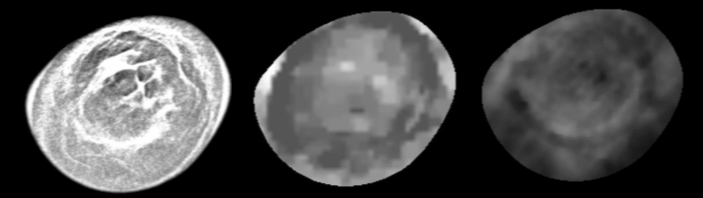
\includegraphics[scale=0.5]{internship_report/images.png}}
\caption{Examples of reflection, sound speed, attenuation images\label{fig:example}}
\end{figure}
I worked in a project called 3D Ultrosound Computer Tomography, shortly USCT. The main goal of the project is development of new image methodology for early breast cancer detection. This type of cancer is one of the most common and dangerous one among women. A breast is not a vital organ, so the most part of patient dies of metastasis, a tumor with size less than 5mm has very low probability of metastasis.  That's why, an early diagnostic of breast cancer significantly increase survival probability of the patient. The USCT team's aim is detection of the tumor with average size small than 5mm. 

The USCT detector is able to produce three different types of images(Pic. \ref{fig:example}):

\begin{enumerate}
\item Reflection - contains general structure
\item Sound speed - map of the soundspeed distribution
\item Attenuation - map of the sound wave's amplitude attenuation
\end{enumerate}

The sound speed and attenuation images give doctors an opportunity to classify lesions precisely, while the reflection's one allows them define type of the structure. I worked on fusion of this three different images into the single one, because it makes an analising easier.(Figure \ref{fig:nicol}
\begin{figure}[H]
\centerline{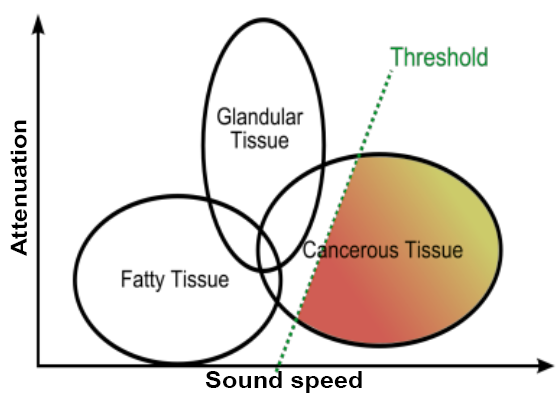
\includegraphics[scale=0.5]{internship_report/nicol}}
\caption{Tumor clasification based on sound speed and attenuation\label{fig:nicol}}
\end{figure}
\subsection{Position description}

3D USCT volumes are converted into stacks of 2D images along specified standard slicing directions used in radiological workflows. They are presented to radiologist using USCT's customized edition of DICOM Viewer, which is based on the ImageJ Framework and the Tudor DICOM Viewer. The position title is Visualization of multimodal 3D USCT volume images. So, the aim of this internship is to explore new intuitive ways of multimodal data visualization, create the prototype of the methods and implements the visualisations in the customized DICOM Viewer. The software should be extended accordingly to allow interactive access to the visualization, e.g. to allow user specified input for setting thresholds, choosing projection directions etc.\\

I also have had my personal goals related with the intnernship:
\begin{itemize}
\item Improve skills on object-oriented programming with Java\footnote{Java is one of the main languages studied in my program at Savonia UAS}improve knowledge of MATLAB
\item Gain experience in digital image processing
\item Get experience in team work on real-life project
\item Learn software development workflow
\end{itemize}

I did not have any expirince in digital image processing befor the internship, but I have had deep undestanding of color theory, visual art and raster graphics and the knowldege helped me a lot.

\subsection{Work description}
\subsubsection{Prototyping}

The most part of my internship I worked on development of new fusion technics for 3D USCT images under supervision of Dr. Hopp. During the first week I made literature research and came up with several idea for realisation of the fusion. After that I made a prototypes for three best of them in MATLAB. The picture \ref{prot} demostrates prototype of HSV Fusion.\\

\begin{figure}
\centerline{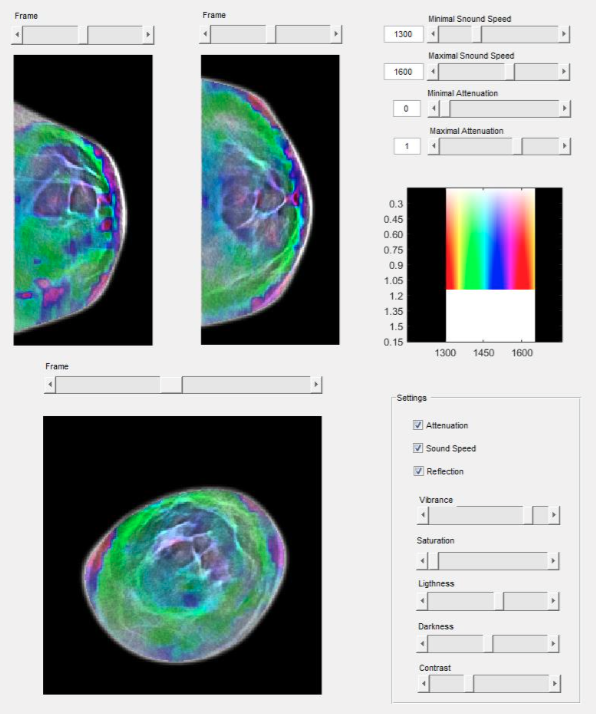
\includegraphics[scale=0.4]{internship_report/pro}}
\caption{MATLAB prototype for HSV Fusion\label{fig:pro}}
\end{figure}
\subsubsection{HSV Fusion}

HSV Fusion was the best solution for fusion of 3D USCT images I founded. The algoright is based on HSV color model. The model devides color of every pixel into three separet components:

\begin{itemize}
\item Hue - keeps chromatic information (how red, green, blue etc. is the pixel)
\item Value - keeps grayscale information (how bright is the pixel)
\item Saturation - keeps an information about saturation of the hue (how the color far away from grayscale)
\end{itemize}

\begin{figure}[H]
\centerline{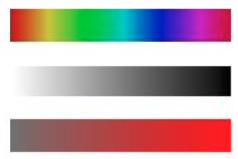
\includegraphics[scale=0.6]{internship_report/hsv}}
\caption{Components of HSV image from to top: Hue, Value, Saturation.\label{fig:hsv}}
\end{figure}

The components are shown on the figure \ref{fig:hsv} The color space of the model can be represented as cylinder, where: altitude is tha Value, saturation is radious from center and angel is hue, look at figure \ref{fig:model}.\\

To get the final result of the fusion the algorithm transfer the image from HSV to RGB color model. The visual representation of the conversion shown at figure \ref{fig:hsv2rgb}.

\begin{figure}[H]
\centerline{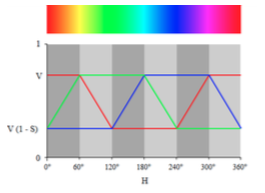
\includegraphics[scale=0.7]{internship_report/hsv2rgb}}
\caption{Visuale representation of HSV to RGB convertions\label{fig:hsv2rgb}}
\end{figure}

\subsubsection{DICOM Viewer realisation}

The prototype was presented to the Software Methods groupe of IPE. The realisation get positive feedback from the team and I started the realisation of the algorithm in DICOM Viewer with ImageJ.\\


The DICOM realisation has a little bit more simple user interface, to make it more understandable for an end user. Sound speed thresholding were added to the final version of fusion, figure \ref{fig:final}.

\begin{figure}
\centerline{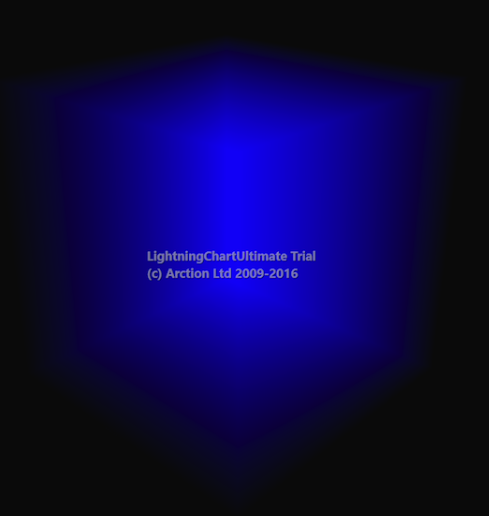
\includegraphics[scale=0.5]{internship_report/final}}
\caption{DICOM Viewer HSV Fusion Menu \label{fig:final}}
\end{figure}

\subsubsection{Re-slicing}

As I mentionet before DICOM Viewer keeps three different stacks of images with different slicing directions for an every breast, but any of this three stacks contains enoght information for visualising of all three slicing directions.\\

\begin{figure}[H]
\centerline{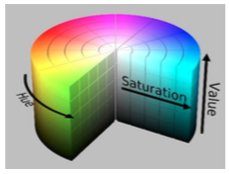
\includegraphics[scale=0.7]{internship_report/model}}
\caption{Model of HSV color space\label{fig:model}}
\end{figure}

My task was to implement the reslicing algorithm whihc allows DICOM Viewer recalculate all three slicing directions from any of them. If density a long different axis is not uniform the algorithm also had to be interpolated data.\\

Re-slicing is very useful feature for DICOM Viewer, because it will tow times reduce size of the database and it will give an opportunity to brows different slice directions of MRI images\footnote{Usually, MRI imgaes has only one slicing direction}.\\

\subsubsection{WebGL Visualisation for USCT}

I was volunteer to take part at development of 3D WebGL Visualisation of USCT data and Dr. Hopp allowed me to join the team. Michael Zapf was responseable for development of the project and the last part of my internship I did under his controll.\\

The vialisation is based on Tomoraycaster 2\footnote{JavaScript framework visualisation of 3D data developed in IPE}. I had to modify the framework to make it work well with USCT data and develop graphical user interface for better representation of the  visulisation.\\

My work started from deployment of Tomoraycaser 2 example for USCT data, the example was able to show the breast structure from reflectional image. After that I started to make an adoptatoin of the shaders to give them an opportunity to handle multimodal data, basicaly I used very same idea as in Fusion, but I also added severl other features to the realisation. The visulisation was quite slow on weak machines, that's why I also worked on optimasetion of the code.\\

\begin{figure}[H]
\centerline{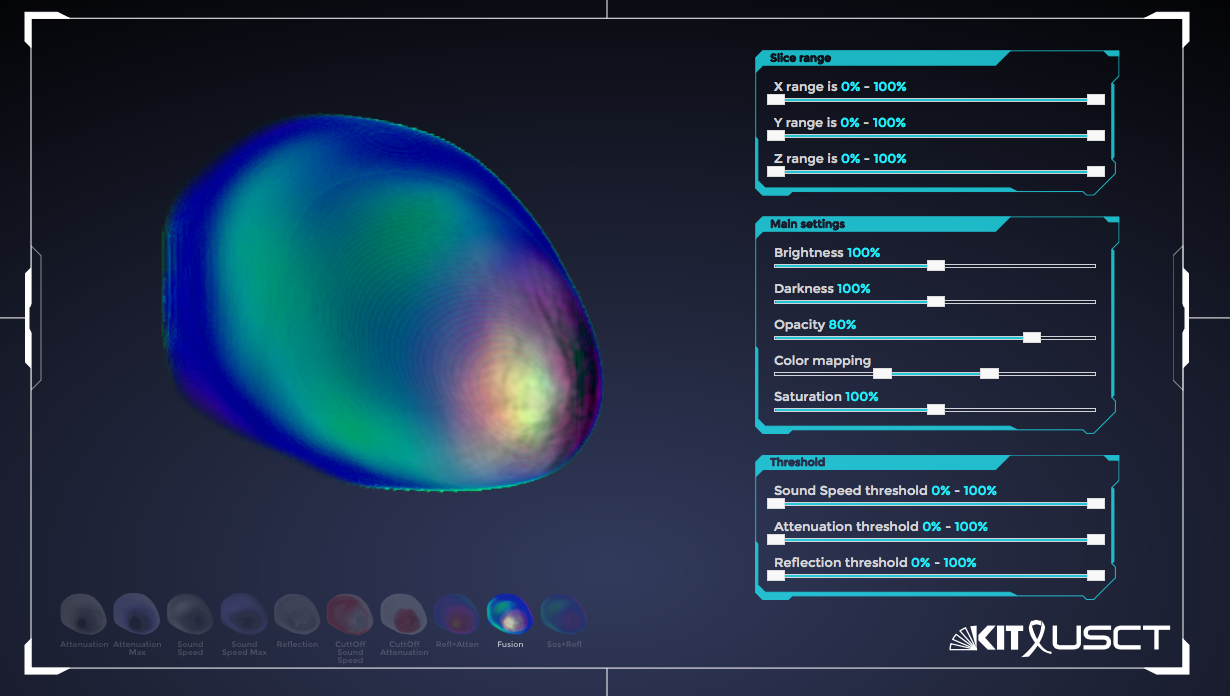
\includegraphics[scale=0.4]{internship_report/usct}}
\caption{Web visualisation for 3D USCT\label{fig:usct}}
\end{figure}

When I finnish my modifications for Tomoraycaster, I started to write the actuall graphical user interface in according with skeleton of the project provided to reslisation me by Nicolas.\\

Our GUI has very complex animation and designe, so we diceded to draw entier website inside huge dynamice SVG image. I used Snap.SVG library to draw SVG images dynamicly inside the webpage. Tomoraycaster and jQuer UI sliders were added to the SVG image as foring object.\\

Final result of the work is 3D visualisation of the USCT data with ten different modes and eleven sliders with different parametrs, pic. \ref{fig:usct}. The visualisation is avaible on this address http://ipepc57.ipe.kit.edu:10002

\subsection{Working place communication}

During the most part of my internship I work under direct supervision of Dr. Torsten Hopp. I recieved the task from my supervisor, asked him for a help then I have had a probmlem and report about current progress. My worked realated with custamization of DICOM Viewer was organised via SVN version controll system, so I worked in my own branch to prevent any additional bugs in the main repository, Dr. Hopp always was able to get my lattes stable code, to check the code style and report about bugs. Every new feature implemented in DICOM Viewer was checked by Dr. Hopp and fixed by me in according with his feedback.\\

Every Wendsday USCT groupe have a meeting. The meeting starts from discussion about current news realted to the project. After that we have had so called "weekly round", durign the "round" every teammember had to report about his/her progress for last week in fron of USCT team on a meeting, durign the report the everyone was able to request help or advise from other ones or help somebody him/herself. \\

At the last part of my internship I worked in cooperation wit Nicolas Tan, he is an expirince web developer reposible for development and maintaince of Tomoraycaster 2, so he was assigned as my mentor for the task. I was very happy to have an opprotunity to work under his guidence, becuase it was prefect chance to improve knowledge in field of web development.\\

During the development of the visualisation I worked in close cooperation with my mentor. We had had discusions about the key issues of the project and made the key dissions toghter. He checked my code and tought me a lot about using of Git and writing a good code. The requerment for the project was developed and controlled by Michael Zapf. Sometimes three of us had a small meetings to make key desisions. Sometimes Michael visited my working place to check current progress, points to bugs and give some advises. 

\section{Conclusion}

I was very satisfied with the internship because I reached my personal goals and in my point of view the task assigned to me was sorted well. In according with the postion goals during the internship I developed new way of visualizing of multimodal USCT data. While implemetetion of the prototype for the algorithm at MATLAB, I improved my knowledge of MATLAB. After that I geined an expirince in object-oriented programming with Java and digital image processing, during integration of the algorithm with DICOM Viewer and work under development of reslicing. I also learned on practise the software development workflow from idea, to prototype and from prototype to implementation and testing.\\

During the second part of my internship I got an expirince in team work on real-life project, I improved my knowledge of tool for team cooperation such as Git version contol system. I also studied in a practice the web development workflow and web development tools like tools like browserify and sass, improved my system administration skills during deployment of the application. Nicolas' guidence helped me to improve my coding style and made my undestanding of JavaScript much deeper.\\

I am very thankful to KIT for this expirince, because I want to build my career in field of digital image processing, visualisation and computer graphics, the work placement gave me first indastieal expirince in this fields, so it means a lot for my future career prospects.\\

I am very thankful to all the people I met during the internship, to the Software Methods groupe of IPE and espectially to Dr. Hopp, Nicolas Tan and Michael Zapf for the guidence and knowledge provided by them.

\end{document}
